\section{Experimental Setup}
\begin{figure}[t]
  \subfloat[]
  {
    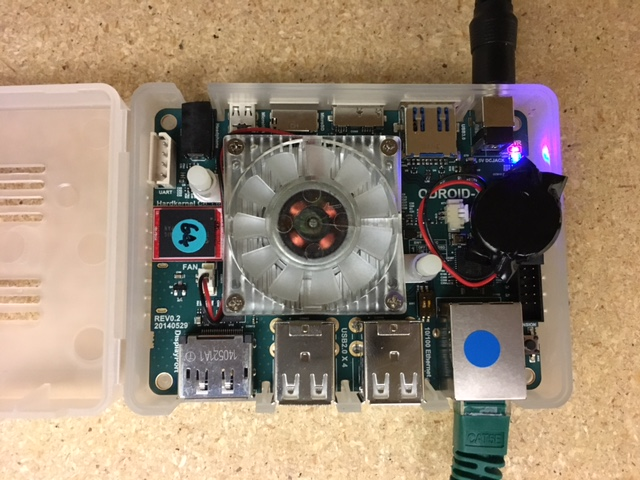
\includegraphics[width=.22\textwidth]{figures/odroid.png}
    \label{fig:odroid}
  }
  \subfloat[]
  {
    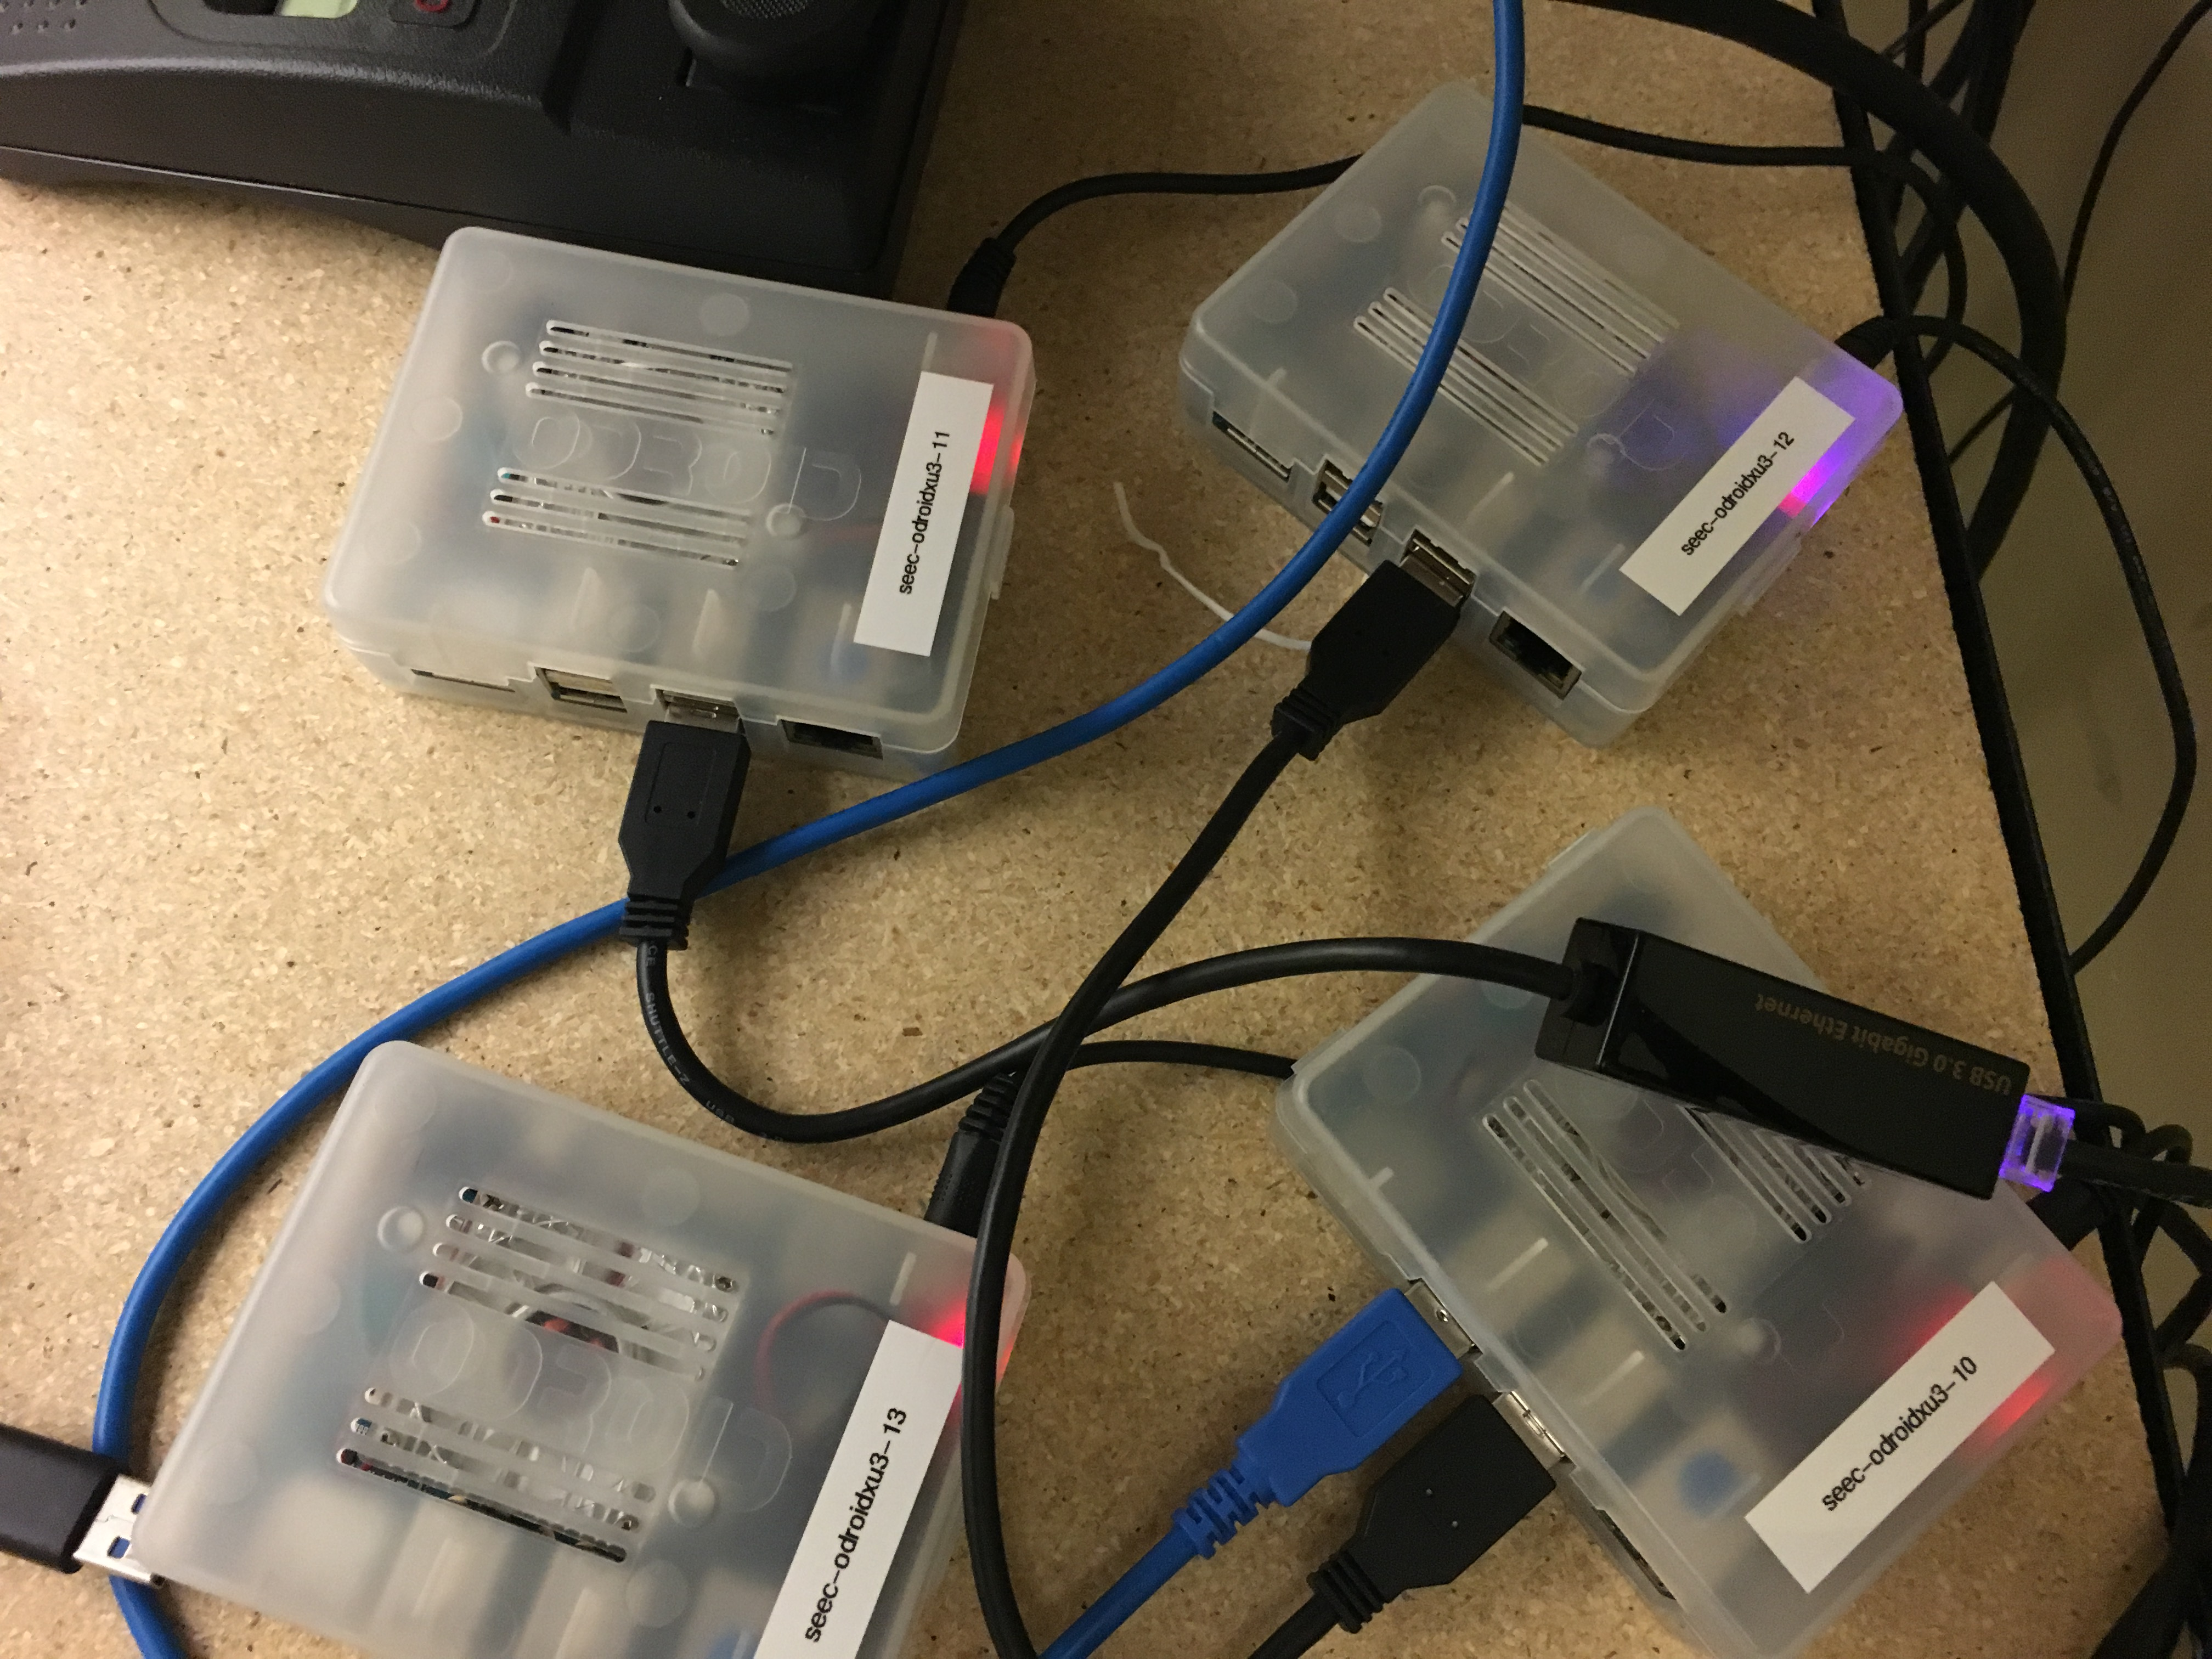
\includegraphics[width=.22\textwidth]{figures/odroidall.png}
    \label{fig:odroid_all}
  }
 \caption{ODROID-XU3 boards used in the evaluation.}
 \label{fig:odroidall}
\end{figure}

\subsection{Platform and Benchmarks}
We run streaming applications on four ODROID-XU3 devices running
Ubuntu 14.04, as shown in \figref{fig:odroidall}. The ODROIDs have
Samsung Exynos 5 Octa processors using the ARM big.LITTLE
architecture.  Each has 19 speed settings for the 4 big cores and 13
for 4 LITTLE cores.  Each board has an on-board power meter updated at
1/4 \ms intervals, this meter captures core, GPU, memory, and flash
drive power.  Each resource configuration (combination of big/LITTLE
cores and clock-speeds) has a different performance and power, which
is application-dependent.

We use 20 benchmarks from different suites including PARSEC \PUNT{
  (\texttt{blackscholes}, \texttt{facesim}, \texttt{ferret},
  \texttt{x264})} \cite{parsec}, Minebench \PUNT{(\texttt{Kmeans},
  \texttt{non fuzzy kmeans \\* (Kmeansnf)})} \cite{minebench}, Rodinia
\PUNT{
  (\texttt{backprop}, \texttt{cfd}, \texttt{nn}, \texttt{lud}, \\*
  \texttt{backprop}, \texttt{bfs})}\cite{rodinia}, and STREAM
\cite{stream}. \figref{fig:application_variety} shows the variety of
workloads indicated by the \emph{lack-of-fit} or the lack of
correlation between frequency and performance.  Applications with high
lack-of-fit do not speed up with increasing frequency, typical of
memory bound applications. Applications with low lack-of-fit do see
increasing performance with increasing clock-speed \cite{powerslope}.
Applications with intermediate lack-of-fit tend to improve with
increasing clock speed up to a point and then see no further
improvement.  Each application has an outer loop which processes one
unit in a data stream (\eg{} a point for \texttt{kmeans} or a frame
for \texttt{x264}). The application signals the completion of
processing a single stream element using a standard API
\cite{icac2010heartbeats}.  Performance targets are specified as
application-specific rates for processing these streams.



\begin{figure}[t]
  \begin{tikzpicture}
\definecolor{s1}{RGB}{228, 26, 28}
\definecolor{s2}{RGB}{55, 126, 184}
\definecolor{s3}{RGB}{77, 175, 74}
\definecolor{s4}{RGB}{152, 78, 163}
\definecolor{s5}{RGB}{255, 127, 0}

\begin{groupplot}[
    group style={
        group name=plots,
        group size=1 by 1,
        xlabels at=edge top,
        xticklabels at=edge top,
        vertical sep=5pt
    },
axis x line* = top,
xlabel near ticks,
major x tick style = transparent,
height=3cm,
width=\columnwidth,
xmin=0,
xmax=9,
enlargelimits=false,
tick align = outside,
tick style={white},
ylabel style={align=center},
ytick=\empty,
xtick=\empty,
xticklabels={},
yticklabels={},
ymin=0,
ymax=1,
]
\nextgroupplot[ylabel={},
y label style={rotate=270},
ylabel shift={12mm},
]
\addplot[thick,solid, color=black] coordinates {(0,1) (22,1)};


\end{groupplot}

\begin{groupplot}[
    group style={
        group name=plots,
        group size=1 by 2,
        xlabels at=edge bottom,
        xticklabels at=edge bottom,
        vertical sep=5pt
    },
axis x line* = bottom,
xlabel near ticks,
major x tick style = transparent,
xlabel={},
height=3cm,
width=\columnwidth,
xmin=0,
xmax=21,
enlargelimits=false,
tick align = outside,
tick style={white},
ylabel style={align=center},
ytick=\empty,
ymin=0,
ymax=0.5,
ytick={0,0.1,0.3,0.5},
yticklabels={,0.1,0.3,0.5},
legend cell align=left, 
legend style={ column sep=1ex },
ymajorgrids,
grid style={dashed},
]


\nextgroupplot[ybar=\pgflinewidth,
bar width=2.0pt,
ylabel={\footnotesize \emph{lack-of-fit} \\ (1-adjustedR2)}, 
ylabel shift={0mm},
xticklabel shift={1pt},
x tick label style={rotate=35, anchor=east},
xtick={1,2,3,4,5,6,7,8,9,10,11,12,13,14,15,16,17,18,19,20,21},
xticklabels={
{\scriptsize $\mathsf{backprop}$},
{\scriptsize $\mathsf{bfs}$},
{\scriptsize $\mathsf{blackscholes}$},
{\scriptsize $\mathsf{bodytrack}$},
{\scriptsize $\mathsf{facesim}$},
{\scriptsize $\mathsf{ferret}$},
{\scriptsize $\mathsf{heartwall}$},
{\scriptsize $\mathsf{hotspot}$},
{\scriptsize $\mathsf{jacobi}$},
{\scriptsize $\mathsf{kmeans}$},
{\scriptsize $\mathsf{kmeansnf}$},
{\scriptsize $\mathsf{lavamd}$},
{\scriptsize $\mathsf{leukocyte}$},
{\scriptsize $\mathsf{lud}$},
{\scriptsize $\mathsf{nw}$},
{\scriptsize $\mathsf{sha}$},
{\scriptsize $\mathsf{srad}$},
{\scriptsize $\mathsf{stream_threads}$},
{\scriptsize $\mathsf{x264-ducks}$},
{\scriptsize $\mathsf{x264-native}$}},
]
\addplot[color=calnp,fill=calnp] table[x index=0,y index=1, col sep=space] {img/image_text/mem-compute.txt};

\end{groupplot}
\end{tikzpicture}
   \vskip -1em
  \caption{\emph{Lack-of-fit} for performance vs clock-speed for a fixed number of cores. Lower value for lack-of-fit indicates a more compute-bound application whereas a higher value indicates a memory bound application.}
  \label{fig:application_variety}
\end{figure}


\subsection{Evaluation Metrics}
\PUNT{
We evaluate learning methods by computing the \emph{accuracy} of the
learned models:
\begin{equation}
\label{eq:accuracy}
accuracy(\hat{\y},\y) = max\left(1 - \frac{\| \hat{\y}-\y \|^2_2 }{\| \y - \bar{\y}\|^2_2},0\right).
\end{equation}
where $\hat{\y}$ represents the predicted performance/power values
and $\y$ is the true value of the power and performance.
}


%\SYSTEM{} uses the model for power and performance and its controller
%actively uses this knowledge to meet the performance target. 
A performance target is a quality-of-service expectation for the
application. We run our applications from 50\% to 90\% performance
targets and evaluate \SYSTEM{} under each constraint. We quantify the
performance reliability using the standard control metric \emph{mean
  absolute percentage error} (MAPE).  If the application processes $n$
stream elements while maintaining a speed of $S$, then its MAPE is:
\begin{equation}
MAPE = 100\% \cdot \frac{1}{n} \sum\limits_{i=1}^{n} max \left( \frac{S - s(i)}{S},0 \right)
\end{equation}
where $S$ is the performance target and $s(i)$ is the performance
observed for $i$th stream element.


%We evaluate energy savings by constructing an oracle.  
We run every application in every resource configuration and record
performance and power for every iteration.  By post-processing this
data we determine the optimal configuration for stream iteration and
performance target. To compare across applications, we normalize
energy:
\begin{equation}
<<<<<<< HEAD
  normalized\,energy = 100\% . \lparen  \frac{e_{measured}}{e_{optimal}}  - 1 \rparen
=======
  normalized\,energy = 100\% . \left( \frac{e_{measured}}{e_{optimal}} - 1 \right)
>>>>>>> 5a87906bd27ff4519722f717b300de4625f6eead
\end{equation}
where $e_{measured}$ is measured energy and $e_{optimal}$ is the optimal energy
produced by our oracle. We subtract 1, so that this metric shows the
percentage of energy over optimal.  \PUNT{ \TODO{Should we multiply
    this by 100, so that it is also a \%?  That seems like a good idea
    -- might as well be consistent across the two metrics.  We don't
    even have to change the data, just the axis labels. } }



\subsection{Points of Comparison}
We compare \SYSTEM{} to a combination of different learning models
and a state-of-art controller based on the \emph{Pace-to-idle (P2I)}
heuristic \cite{kim-cpsna}.  Pace-to-idle is proven never to be worse
than race-to-idle and often provides as much as $2\times$ energy
savings, but requires application-specific knowledge to implement.
Pace-to-idle processes a stream element in the most energy-efficient
configuration and then transitions to a low-power sleep state until
the next job is ready.  We compare \SYSTEM{}'s performance and energy
with:
\begin{enumerate}
\item \textit{Online}: observes the new application in small number of
  configurations then performs polynomial multivariate regression to
  estimate unobserved configurations' performance and power. \PUNT{We
    use the \textit{Online} learning model in combination with
    \emph{Pace-to-idle (P2I)} heuristic.}
\item \textit{Offline}: does not observe any values for the current
  application -- instead using previously observed applications to
  estimate power and performance as a linear regression. \PUNT{We use
    the \textit{Offline} learning model in combination with
    \emph{Pace-to-idle (P2I)} heuristic.}
\item \textit{LEO}: is a hierarchical Bayesian learner \cite{LEO}.
\item \textit{POET}: a state-of-the-art, control system designed to
  meet application performance with minimal energy \cite{POET}.  POET
  requires users to specify a model.  We use POET with the model
  produced by the \emph{Offline} learner.
\item \textit{CALOREE-NP}: is CALOREE with pole set to 0, which we
  include to show the importance of informing the controller of the
  confidence interval and model variance.
\end{enumerate}

In all cases that require prior knowledge, we ensure that knowledge of
the application under test is never included in that set of prior
knowledge.  Specifically, we use leave-one-out cross validation: to
test application $x$, we form a set of all other applications, train
the models, and then test on $x$.


\section{Experimental Evaluation}
\PUNT {We evaluate \SYSTEM{}'s ability to deliver requested
  performance with near-optimal energy. We first examine a
  single-application scenario, where each application is run by
  itself.  We then consider a multi-application scenario where each
  application is run and then, halfway through, a second random
  application is launched, testing the ability to deliver performance
  in a changing environment.  We then examine other dynamic scenarios
  where application inputs or behavior changes during application
  execution.}

\subsection{Performance and Energy for Single App}
%Setup
\begin{figure}[!h]
\centering
  \begin{tikzpicture}
\begin{centering}

\begin{groupplot}[
    group style={
        group name=plots,
        group size=2 by 1,
        xlabels at=edge bottom,
        xticklabels at=edge bottom,
        horizontal sep=50pt
    },
height=3cm,
width=0.45\columnwidth,
%xmajorgrids,
ymajorgrids,
grid style={dashed},
xmin=-6,
xmax=8,
yticklabel pos=left,
enlargelimits=false,
tick align = outside,
tick style={white},
%xticklabel shift={5pt},
%yticklabel shift={-5pt},
%ylabel shift={-2pt},
ylabel style={align=center},
unbounded coords=jump,
]

\nextgroupplot[ybar=7.0pt,
ylabel={\footnotesize \% MAPE \\ {\scriptsize (lower is better)}},
ylabel shift={0mm},
bar width=3.0pt,
ytick={0,3,6,9,12,15},
yticklabels={,3,6,9,12,15},
ymin=0,
ymax=15,
yticklabel style={font=\footnotesize},
x tick label style={rotate=35, anchor=east},
xtick={-5.5,-2.66,0.33,2.66,5,7},
xticklabels={
  {\tiny $\mathsf{Online}$},
  {\tiny $\mathsf{Offline}$},
  {\tiny $\mathsf{LEO}$},
  {\tiny $\mathsf{POET}$},
  {\tiny $\mathsf{CALOREE-NP}$},
  {\tiny $\mathsf{CALOREE}$},
 },
]

\addplot[color=on,fill=on]         table[x index=0,y index=2, col sep=space] {img/single-app-data-perf.txt};
 \addplot[color=off,fill=off]         table[x index=0,y index=3, col sep=space] {img/single-app-data-perf.txt};
 \addplot[color=leo,fill=leo]         table[x index=0,y index=4, col sep=space] {img/single-app-data-perf.txt};
 \addplot[color=poet,fill=poet]       table[x index=0,y index=5, col sep=space] {img/single-app-data-perf.txt};
 \addplot[color=calnp, fill=calnp]     table[x index=0,y index=6, col sep=space] {img/single-app-data-perf.txt};
 \addplot[color=cal,fill=cal]         table[x index=0,y index=7, col sep=space] {img/single-app-data-perf.txt};

\nextgroupplot[ybar=7.0pt,
ylabel={\footnotesize \% Energy \\ {\scriptsize (lower is better)}},
ylabel shift={0mm},
bar width=3.0pt,
ytick={0,5,10,15,20,25},
yticklabels={,5,10,15,20,25},
ymin=0,
ymax=25,
yticklabel style={font=\footnotesize},
xlabel near ticks,
x tick label style={rotate=35, anchor=east},
xtick={-5.5,-2.66,0.33,2.66,5,7},
xticklabels={
  {\tiny $\mathsf{Online}$},
  {\tiny $\mathsf{Offline}$},
  {\tiny $\mathsf{LEO}$},
  {\tiny $\mathsf{POET}$},
  {\tiny $\mathsf{CALOREE-NP}$},
  {\tiny $\mathsf{CALOREE}$},
 },
]

\addplot[color=on, fill=on]           table[x index=0,y index=2, col sep=space] {img/single-app-data-power.txt};
 \addplot[color=off, fill=off]         table[x index=0,y index=3, col sep=space] {img/single-app-data-power.txt};
 \addplot[color=leo, fill=leo]         table[x index=0,y index=4, col sep=space] {img/single-app-data-power.txt};
 \addplot[color=poet,fill=poet]       table[x index=0,y index=5, col sep=space] {img/single-app-data-power.txt};
 \addplot[color=calnp,fill=calnp]     table[x index=0,y index=6, col sep=space] {img/single-app-data-power.txt};
 \addplot[color=cal,fill=cal]         table[x index=0,y index=7, col sep=space] {img/single-app-data-power.txt};

\end{groupplot}
\end{centering}
\end{tikzpicture}

   \vskip -.5em
  \caption{Summary data for single-app scenario.}
  \label{fig:single-sum}
\end{figure}

We set a range of performance targets from 50-90\% of the maximum
achievable performance and measure the MAPE (performance error) and
energy efficiency (energy over optimal) for all points of comparison.
\figref{fig:single-sum} represents the summary results as an average
error across all targets for single application scenario.
\figsref{fig:single-perf}{fig:single-energy} show the detailed results
for the 50, 70, and 90\% targets\footnote{We would happily provide
  that data anonymously through the PC chair if a reviewer finds it
  important to the evaluation}, others are similar but elided for
space.  The benchmarks are shown on the x-axis; the y-axis show MAPE
and the normalized energy, respectively.  \SYSTEM{} has lower MAPE and
energy consumption than the baseline algorithms.


\begin{figure*}[!t]
  \begin{tikzpicture}
%\pgfplotstableread[col sep=space]{img/image_text/dyn-mape-0.5-v2.txt}{\datatablefive}
\pgfplotstableread[col sep=space]{img/image_text/dyn-lat-0.60-v3.txt}{\datatablesixty}
\pgfplotstableread[col sep=space]{img/image_text/dyn-lat-0.75-v3.txt}{\datatableseventyfive}
\pgfplotstableread[col sep=space]{img/image_text/dyn-lat-0.90-v3.txt}{\datatableninty}
\begin{groupplot}[
    group style={
        group name=plots,
        group size=1 by 3,
        xlabels at=edge bottom,
        xticklabels at=edge bottom,
        vertical sep=5pt
    },
axis x line* = bottom,
xlabel near ticks,
major x tick style = transparent,
xlabel={},
height=2.8cm,
width=0.88\textwidth,
xmin=0,
xmax=23,
enlargelimits=false,
tick align = outside,
tick style={white},
ylabel style={align=center},
ytick=\empty,
ymin=0,
ymax=30,
ytick={0,5,10,15,20},
yticklabels={,5,10,15,20},
legend cell align=left, 
legend style={ column sep=1ex },
ymajorgrids,
grid style={dashed},
]


\nextgroupplot[ybar=\pgflinewidth,
ylabel shift={0mm},
bar width=2.0pt,
legend entries = {{$\mathsf{Race-to-idle}$},
{$\mathsf{Netflix}$},
{$\mathsf{HBM}$},
{$\mathsf{POET}$},
{$\mathsf{CALOREE-HBM}$}},
legend style={draw=none, legend columns=6,at={(.5,1.7)},anchor=north},
ymin=0,
ymax=20,
ytick={0.0,5.0,10.0,15.0,20.0},
yticklabels={,5.0,10.0,15.0},
]

\addplot[color=RACE, fill=RACE]       table[x index=0,y index=3] {\datatablesixty};
\addplot[color=NETFLIX, fill=NETFLIX]     table[x index=0,y index=6] {\datatablesixty};
\addplot[color=HBM, fill=HBM]   table[x index=0,y index=7] {\datatablesixty};
\addplot[color=POET, fill=POET] table[x index=0,y index=9] {\datatablesixty};
\addplot[color=CALOREE-HBM, fill=CALOREE-HBM]     table[x index=0,y index=13] {\datatablesixty};
                                

\nextgroupplot[ybar=\pgflinewidth,
ylabel={\footnotesize MAPE  {\scriptsize (lower is better)}},
ylabel shift={0mm},
bar width=2.0pt,
ymin=0,
ymax=30,
ytick={0.0,10.0,20.0,30.0},
yticklabels={,10.0,20.0,30.0},
]

%\addplot[color=RACE,fill=RACE] table[x index=0,y index=4] {\datatableseventyfive};
%\addplot[color=HBM,fill=HBM]       table[x index=0,y index=7] {\datatableseventyfive};
%\addplot[color=ADAPT-CONTROL,fill=ADAPT-CONTROL] table[x index=0,y index=9] {\datatableseventyfive};
%\addplot[color=CALOREE-NP,fill=CALOREE-NP]   table[x index=0,y index=10] {\datatableseventyfive};
%\addplot[color=HBM-ADAPT,fill=HBM-ADAPT]       table[x index=0,y index=13] {\datatableseventyfive};
\addplot[color=RACE, fill=RACE]       table[x index=0,y index=3] {\datatableseventyfive};
\addplot[color=NETFLIX, fill=NETFLIX]     table[x index=0,y index=6] {\datatableseventyfive};
\addplot[color=HBM, fill=HBM]   table[x index=0,y index=7] {\datatableseventyfive};
\addplot[color=POET, fill=POET] table[x index=0,y index=9] {\datatableseventyfive};
\addplot[color=CALOREE-HBM, fill=CALOREE-HBM]     table[x index=0,y index=13] {\datatableseventyfive};

\nextgroupplot[ybar=\pgflinewidth,
bar width=2.0pt,
ylabel shift={0mm},
xticklabel shift={0pt},
ymin=0,
ymax=30,
ytick={0.0,10.0,20.0,30.0},
yticklabels={,10.0,20.0,30.0},
x tick label style={rotate=35, anchor=east},
xtick={1,2,3,4,5,6,7,8,9,10,11,12,13,14,15,16,17,18,19,20,21,22},
xticklabels={
{\scriptsize $\mathsf{backprop}$},
{\scriptsize $\mathsf{bfs}$},
{\scriptsize $\mathsf{blackscholes}$},
{\scriptsize $\mathsf{bodytrack}$},
{\scriptsize $\mathsf{facesim}$},
{\scriptsize $\mathsf{ferret}$},
{\scriptsize $\mathsf{heartwall}$},
{\scriptsize $\mathsf{hotspot}$},
{\scriptsize $\mathsf{jacobi}$},
{\scriptsize $\mathsf{kmeans}$},
{\scriptsize $\mathsf{kmeansnf}$},
{\scriptsize $\mathsf{lavamd}$},
{\scriptsize $\mathsf{leukocyte}$},
{\scriptsize $\mathsf{lud}$},
{\scriptsize $\mathsf{nw}$},
{\scriptsize $\mathsf{sha}$},
{\scriptsize $\mathsf{srad}$},
{\scriptsize $\mathsf{stream}$},
{\scriptsize $\mathsf{stream_threads}$},
{\scriptsize $\mathsf{x264-ducks}$},
{\scriptsize $\mathsf{x264-native}$},
{\scriptsize $\mathsf{Average}$}},
]

\addplot[color=RACE, fill=RACE]       table[x index=0,y index=3] {\datatableninty};
\addplot[color=NETFLIX, fill=NETFLIX]     table[x index=0,y index=6] {\datatableninty};
\addplot[color=HBM, fill=HBM]   table[x index=0,y index=7] {\datatableninty};
\addplot[color=POET, fill=POET] table[x index=0,y index=9] {\datatableninty};
\addplot[color=CALOREE-HBM, fill=CALOREE-HBM]     table[x index=0,y index=13] {\datatableninty};

\end{groupplot}
\begin{groupplot}[
    group style={
        group name=plots,
        group size=1 by 6,
        xlabels at=edge top,
        xticklabels at=edge top,
        vertical sep=5pt
    },
axis x line* = top,
xlabel near ticks,
major x tick style = transparent,
height=2.8cm,
width=0.88\textwidth,
xmin=0,
xmax=9,
enlargelimits=false,
tick align = outside,
tick style={white},
ylabel style={align=center},
ytick=\empty,
xtick=\empty,
xticklabels={},
yticklabels={},
ymin=0,
ymax=1,
]

\nextgroupplot[
ylabel shift={12mm},
ylabel style={rotate=270},
ylabel={$\mathsf{60\%}$},
]
\addplot[thick,solid, color=black] coordinates {(0,1) (22,1)};


\nextgroupplot[
ylabel shift={12mm},
ylabel={$\mathsf{75\%}$},
ylabel style={rotate=270},
]
\addplot[thick,solid, color=black] coordinates {(0,1) (22,1)};


\nextgroupplot[
ylabel shift={12mm},
ylabel={$\mathsf{90\%}$},
y label style={rotate=270},
]
\addplot[thick,solid, color=black] coordinates {(0,1) (22,1)};

\end{groupplot}

\end{tikzpicture}
   \vskip -.5em
  \caption{Comparison of application performance error for single application scenario.}
  \label{fig:single-perf}
\end{figure*}


\begin{figure*}[!t]
  
\begin{tikzpicture}

\pgfplotstableread[col sep=tab]{img/image_text/wcet-eff-1.0.txt}{\datatableninty}
\begin{groupplot}[
    group style={
        group name=plots,
        group size=1 by 1,
        xlabels at=edge bottom,
        xticklabels at=edge bottom,
        vertical sep=5pt
    },
axis x line* = bottom,
xlabel near ticks,
major x tick style = transparent,
xlabel={},
height=3.0cm,
width=0.95\textwidth,
xmin=0,
xmax=15,
enlargelimits=false,
tick align = outside,
tick style={white},
ylabel style={align=center},
ytick=\empty,
ymin=0,
ymax=15,
ytick={0,5,10,15,20},
yticklabels={,5,10,15,20},
ylabel={\tiny Energy Above \\ {\tiny Optimal (\%)} \\ {\tiny (lower is better)}},
legend cell align=left, 
legend style={ column sep=1ex },
ymajorgrids,
grid style={dashed},
]

\nextgroupplot[ybar=\pgflinewidth,
bar width=4.0pt,
ylabel shift={0mm},
xticklabel shift={0pt},
ymin=0,
ymax=90,
ytick={0.0,30.0,60.0,90.0},
yticklabels={,30.0,60.0,90.0},
x tick label style={rotate=35, anchor=east},
xtick={1,2,3,4,5,6,7,8,9,10,11,12,13,14},
xticklabels={
{\tiny $\mathsf{bodytrack}$},
{\tiny $\mathsf{facesim}$},
{\tiny $\mathsf{ferret}$},
{\tiny $\mathsf{heartwall}$},
{\tiny $\mathsf{kmeans}$},
{\tiny $\mathsf{leukocyte}$},
{\tiny $\mathsf{lud}$},
{\tiny $\mathsf{radar}$},
{\tiny $\mathsf{sha}$},
{\tiny $\mathsf{srad}$},
{\tiny $\mathsf{stream}$},
{\tiny $\mathsf{x264-ducks}$},
{\tiny $\mathsf{x264-native}$},
{\tiny $\mathsf{Average}$}},
]

\addplot[color=black, fill=RACE]       table[x index=0,y index=3] {\datatableninty};
\addplot[color=black, fill=NETFLIX]     table[x index=0,y index=6] {\datatableninty};
\addplot[color=black, fill=HBM]   table[x index=0,y index=7] {\datatableninty};
\addplot[color=black, fill=POET] table[x index=0,y index=9] {\datatableninty};
\addplot[color=black, fill=CALOREE-HBM]     table[x index=0,y index=13] {\datatableninty};

\end{groupplot}


\end{tikzpicture}

   \vskip -.5em
  \caption{Comparison of application energy consumption for single application scenario.}
  \label{fig:single-energy}
\end{figure*}


\PUNT{Across all applications and
targets, the online model produces an average error of 9.8\%, the
offline: 3.6\%, LEO: 8.0\%, POET: 10.4\%, CALOREE-NP: 6.4\% and
\SYSTEM{}: 0.5\%.  \SYSTEM{} clearly produces a dramatic error
reduction compared to prior approaches -- in fact, \SYSTEM{} MAPE is
generally not visible on the charts.

Regarding energy consumption, the online model requires an average of
21\% more energy than optimal, offline: 15\%, LEO: 14\%, POET: 24\%,
CALOREE-NP: 9.5\%, and \SYSTEM{}: 4.1\%.  }
\SYSTEM{} provides a
significant energy savings even when compared to state-of-the-art learning
or control approaches.  The reason is that the combination is
complementary: LEO produces accurate models while control both can
correct small errors in those models and adapt to dynamic changes in
behavior.  Even without a pole, CALOREE would improve over the
state-of-the-art, but when the pole is included, the results are a
significant improvement.






%In addition to providing better average case behavior, \SYSTEM{}
%provides significantly better worst case behavior.  


\subsection{Performance and Energy for Multiple Apps}
\begin{figure}[!h]
\centering
  \begin{tikzpicture}
\begin{centering}

\begin{groupplot}[
    group style={
        group name=plots,
        group size=2 by 1,
        xlabels at=edge bottom,
        xticklabels at=edge bottom,
        horizontal sep=50pt
    },
height=3cm,
width=0.45\columnwidth,
%xmajorgrids,
ymajorgrids,
grid style={dashed},
xmin=-6,
xmax=8,
yticklabel pos=left,
enlargelimits=false,
tick align = outside,
tick style={white},
%xticklabel shift={5pt},
%yticklabel shift={-5pt},
%ylabel shift={-2pt},
ylabel style={align=center},
unbounded coords=jump,
]

\nextgroupplot[ybar=7.0pt,
ylabel={\footnotesize \% MAPE \\ {\scriptsize (lower is better)}},
ylabel shift={0mm},
bar width=3.0pt,
ytick={0,5,10,15,20,25},
yticklabels={,5,10,15,20,25},
ymin=0,
ymax=25,
yticklabel style={font=\footnotesize},
x tick label style={rotate=35, anchor=east},
xtick={-5.5,-2.66,0.33,2.66,5,7},
xticklabels={
  {\tiny $\mathsf{Online}$},
  {\tiny $\mathsf{Offline}$},
  {\tiny $\mathsf{LEO}$},
  {\tiny $\mathsf{POET}$},
  {\tiny $\mathsf{CALOREE-NP}$},
  {\tiny $\mathsf{CALOREE}$},
 },
]

\addplot[color=on,fill=on]         table[x index=0,y index=2, col sep=space] {img/multi-app-data-perf.txt};
 \addplot[color=off,fill=off]         table[x index=0,y index=3, col sep=space] {img/multi-app-data-perf.txt};
 \addplot[color=leo,fill=leo]         table[x index=0,y index=4, col sep=space] {img/multi-app-data-perf.txt};
 \addplot[color=poet,fill=poet]       table[x index=0,y index=5, col sep=space] {img/multi-app-data-perf.txt};
 \addplot[color=calnp, fill=calnp]     table[x index=0,y index=6, col sep=space] {img/multi-app-data-perf.txt};
 \addplot[color=cal,fill=cal]         table[x index=0,y index=7, col sep=space] {img/multi-app-data-perf.txt};

\nextgroupplot[ybar=7.0pt,
ylabel={\footnotesize \% Energy \\ {\scriptsize (lower is better)}},
ylabel shift={0mm},
bar width=3.0pt,
ytick={0,5,10,15,20,25},
yticklabels={,5,10,15,20,25},
ymin=0,
ymax=25,
yticklabel style={font=\footnotesize},
xlabel near ticks,
x tick label style={rotate=35, anchor=east},
xtick={-5.5,-2.66,0.33,2.66,5,7},
xticklabels={
  {\tiny $\mathsf{Online}$},
  {\tiny $\mathsf{Offline}$},
  {\tiny $\mathsf{LEO}$},
  {\tiny $\mathsf{POET}$},
  {\tiny $\mathsf{CALOREE-NP}$},
  {\tiny $\mathsf{CALOREE}$},
 },
]

\addplot[color=on, fill=on]           table[x index=0,y index=2, col sep=space] {img/multi-app-data-power.txt};
 \addplot[color=off, fill=off]         table[x index=0,y index=3, col sep=space] {img/multi-app-data-power.txt};
 \addplot[color=leo, fill=leo]         table[x index=0,y index=4, col sep=space] {img/multi-app-data-power.txt};
 \addplot[color=poet,fill=poet]       table[x index=0,y index=5, col sep=space] {img/multi-app-data-power.txt};
 \addplot[color=calnp,fill=calnp]     table[x index=0,y index=6, col sep=space] {img/multi-app-data-power.txt};
 \addplot[color=cal,fill=cal]         table[x index=0,y index=7, col sep=space] {img/multi-app-data-power.txt};

\end{groupplot}
\end{centering}
\end{tikzpicture}

   \vskip -.5em
  \caption{Summary data for multi-app scenario.}
  \label{fig:multi-sum}
\end{figure}

We again launch each benchmark with a performance target (using the
same targets as the prior study).  Halfway through execution, we start
another application randomly drawn from our benchmark set, which we
bind to one big core.  Launching this second application changes
performance and power consumption.  Delivering performance to the
original application in this dynamic scenario tests the ability to
react to environmental changes.

\figref{fig:multi-sum} summarizes the results as an average error
across all targets for multiple application scenario.
\figsref{fig:multi-perf}{fig:multi-energy} shows the results.  The
90\% target is generally not reachable in this scenario as it would
require the controlled application to have exclusive use of all big
cores.  \SYSTEM{} again has lower MAPE than the baseline algorithms.


\PUNT{
Across all applications and targets, the online model produces an
average error of 21\%, the offline: 24\%, LEO: 19\%, POET: 7.4\%,
CALOREE-NP: 11\%, and \SYSTEM{}: 2.8\%. \SYSTEM{} is also more energy
efficient than the baseline algorithms. Across all applications and
targets, the average normalized energy for online model is 22\%, the
offline: 21\%, LEO: 17\%, POET: 34\%, CALOREE-NP: 13\%, and \SYSTEM{}:
8.5\%.
}
POET and \SYSTEM{} provide more reliable performance because they are
specifically designed to handle system dynamics.  \SYSTEM{}, however,
does significantly better than POET in the worst case because the HBM
produces more robust models.  Again, the results show the benefits of
incorporating model variance into the controller's pole calculation.


\begin{figure*}[htp!]
  \begin{tikzpicture}


\begin{groupplot}[
    group style={
        group name=plots,
        group size=1 by 3,
        xlabels at=edge bottom,
        xticklabels at=edge bottom,
        vertical sep=5pt
    },
axis x line* = bottom,
xlabel near ticks,
major x tick style = transparent,
xlabel={},
height=2.8cm,
width=0.88\textwidth,
xmin=0,
xmax=23,
enlargelimits=false,
tick align = outside,
tick style={white},
ylabel style={align=center},
ytick=\empty,
ymin=0,
ymax=30,
ytick={0,5,10,15,20},
yticklabels={,5,10,15,20},
legend cell align=left, 
legend style={ column sep=1ex },
ymajorgrids,
grid style={dashed},
]



\nextgroupplot[ybar=\pgflinewidth,
ylabel shift={0mm},
bar width=2.0pt,
legend entries = {{$\mathsf{Online}$},{$\mathsf{Offline}$},{$\mathsf{LEO}$},{$\mathsf{POET}$},{$\mathsf{\SYSTEM{}-NP}$},{$\mathsf{\SYSTEM{}}$}},
legend style={draw=none,legend columns=6,at={(.5,1.7)},anchor=north},
ymin=0,
ymax=20,
ytick={0.0,5.0,10.0,15.0,20.0},
yticklabels={,5.0,10.0,15.0},
]

\addplot[color=on,fill=on]  table[x index=0,y index=3, col sep=space] {img/image_text/ma-err-0.5-v2.txt};
\addplot[color=off,fill=off]  table[x index=0,y index=4, col sep=space] {img/image_text/ma-err-0.5-v2.txt};
\addplot[color=leo,fill=leo]  table[x index=0,y index=5, col sep=space] {img/image_text/ma-err-0.5-v2.txt};
\addplot[color=poet,fill=poet]  table[x index=0,y index=6, col sep=space] {img/image_text/ma-err-0.5-v2.txt};
\addplot[color=calnp,fill=calnp]  table[x index=0,y index=7, col sep=space] {img/image_text/ma-err-0.5-v2.txt};
\addplot[color=cal,fill=cal]  table[x index=0,y index=8, col sep=space] {img/image_text/ma-err-0.5-v2.txt};

\nextgroupplot[ybar=\pgflinewidth,
ylabel={\footnotesize MAPE  {\scriptsize (lower is better)}},
ylabel shift={0mm},
bar width=2.0pt,
ymin=0,
ymax=30,
ytick={0.0,10.0,20.0,30.0},
yticklabels={,10.0,20.0,30.0},
]

\addplot[color=on,fill=on]  table[x index=0,y index=3, col sep=space] {img/image_text/ma-err-0.7-v2.txt};
\addplot[color=off,fill=off]  table[x index=0,y index=4, col sep=space] {img/image_text/ma-err-0.7-v2.txt};
\addplot[color=leo,fill=leo]  table[x index=0,y index=5, col sep=space] {img/image_text/ma-err-0.7-v2.txt};
\addplot[color=poet,fill=poet]  table[x index=0,y index=6, col sep=space] {img/image_text/ma-err-0.7-v2.txt};
\addplot[color=calnp,fill=calnp]  table[x index=0,y index=7, col sep=space] {img/image_text/ma-err-0.7-v2.txt};
\addplot[color=cal,fill=cal]  table[x index=0,y index=8, col sep=space] {img/image_text/ma-err-0.7-v2.txt};

\nextgroupplot[ybar=\pgflinewidth,
bar width=2.0pt,
ylabel shift={0mm},
xticklabel shift={0pt},
ymin=0,
ymax=30,
ytick={0.0,10.0,20.0,30.0},
yticklabels={,10.0,20.0,30.0},
x tick label style={rotate=35, anchor=east},
xtick={1,2,3,4,5,6,7,8,9,10,11,12,13,14,15,16,17,18,19,20,21,22},
xticklabels={
{\scriptsize $\mathsf{backprop}$},
{\scriptsize $\mathsf{bfs}$},
{\scriptsize $\mathsf{blackscholes}$},
{\scriptsize $\mathsf{bodytrack}$},
{\scriptsize $\mathsf{facesim}$},
{\scriptsize $\mathsf{ferret}$},
{\scriptsize $\mathsf{heartwall}$},
{\scriptsize $\mathsf{hotspot}$},
{\scriptsize $\mathsf{jacobi}$},
{\scriptsize $\mathsf{kmeans}$},
{\scriptsize $\mathsf{kmeansnf}$},
{\scriptsize $\mathsf{lavamd}$},
{\scriptsize $\mathsf{leukocyte}$},
{\scriptsize $\mathsf{lud}$},
{\scriptsize $\mathsf{nw}$},
{\scriptsize $\mathsf{sha}$},
{\scriptsize $\mathsf{srad}$},
{\scriptsize $\mathsf{stream}$},
{\scriptsize $\mathsf{stream_threads}$},
{\scriptsize $\mathsf{x264-ducks}$},
{\scriptsize $\mathsf{x264-native}$},
{\scriptsize $\mathsf{\mathbf{Average}}$}},
]

\addplot[color=on,fill=on]  table[x index=0,y index=3, col sep=space] {img/image_text/ma-err-0.9-v2.txt};
\addplot[color=off,fill=off]  table[x index=0,y index=4, col sep=space] {img/image_text/ma-err-0.9-v2.txt};
\addplot[color=leo,fill=leo]  table[x index=0,y index=5, col sep=space] {img/image_text/ma-err-0.9-v2.txt};
\addplot[color=poet,fill=poet]  table[x index=0,y index=6, col sep=space] {img/image_text/ma-err-0.9-v2.txt};
\addplot[color=calnp,fill=calnp]  table[x index=0,y index=7, col sep=space] {img/image_text/ma-err-0.9-v2.txt};
\addplot[color=cal,fill=cal]  table[x index=0,y index=8, col sep=space] {img/image_text/ma-err-0.9-v2.txt};

\end{groupplot}
\begin{groupplot}[
    group style={
        group name=plots,
        group size=1 by 6,
        xlabels at=edge top,
        xticklabels at=edge top,
        vertical sep=5pt
    },
axis x line* = top,
xlabel near ticks,
major x tick style = transparent,
height=2.8cm,
width=0.88\textwidth,
xmin=0,
xmax=9,
enlargelimits=false,
tick align = outside,
tick style={white},
ylabel style={align=center},
ytick=\empty,
xtick=\empty,
xticklabels={},
yticklabels={},
ymin=0,
ymax=1,
]

\nextgroupplot[
ylabel shift={12mm},
ylabel style={rotate=270},
ylabel={$\mathsf{50\%}$},
]
\addplot[thick,solid, color=black] coordinates {(0,1) (22,1)};

\nextgroupplot[
ylabel shift={12mm},
ylabel={$\mathsf{70\%}$},
y label style={rotate=270},
]
\addplot[thick,solid, color=black] coordinates {(0,1) (22,1)};

\nextgroupplot[
ylabel shift={12mm},
ylabel={$\mathsf{90\%}$},
y label style={rotate=270},
]
\addplot[thick,solid, color=black] coordinates {(0,1) (22,1)};

\end{groupplot}
\end{tikzpicture}
   \vskip -.5em
  \caption{Comparison of application performance error for multiple application scenario.}
  \label{fig:multi-perf}
\end{figure*}

\begin{figure*}[!t]
  \begin{tikzpicture}
%\pgfplotstableread[col sep=space]{img/image_text/ma-eff-0.60-v4.txt}{\datatablesixty}
%\pgfplotstableread[col sep=space]{img/image_text/ma-eff-0.75-v4.txt}{\datatableseventy}
\pgfplotstableread[col sep=space]{img/image_text/wcet-ma-eff-1.0.txt}{\datatableeighty}
\begin{groupplot}[
    group style={
        group name=plots,
        group size=1 by 1,
        xlabels at=edge bottom,
        xticklabels at=edge bottom,
        vertical sep=5pt
    },
axis x line* = bottom,
xlabel near ticks,
major x tick style = transparent,
xlabel={},
height=3.0cm,
width=0.95\textwidth,
xmin=0,
xmax=15,
enlargelimits=false,
tick align = outside,
tick style={white},
ylabel style={align=center},
ytick=\empty,
ymin=0,
ymax=30,
ytick={0,5,10,15,20},
yticklabels={,5,10,15,20},
legend cell align=left,
legend style={ column sep=1ex },
ymajorgrids,
grid style={dashed},
]

\nextgroupplot[ybar=\pgflinewidth,
bar width=3.0pt,
ylabel shift={0mm},
ylabel={\tiny Energy Above Optimal \\ {\tiny (lower is better)}},
xticklabel shift={0pt},
ymin=0,
ymax=90,
ytick={0.0,30.0,60.0,90.0},
yticklabels={,30.0,60.0,90.0},
x tick label style={rotate=35, anchor=east},
xtick={1,2,3,4,5,6,7,8,9,10,11,12,13,14,15,16,17,18,19,20,21,22},
xticklabels={
{\scriptsize $\mathsf{bodytrack}$},
{\scriptsize $\mathsf{facesim}$},
{\scriptsize $\mathsf{ferret}$},
{\scriptsize $\mathsf{heartwall}$},
{\scriptsize $\mathsf{kmeans}$},
{\scriptsize $\mathsf{leukocyte}$},
{\scriptsize $\mathsf{lud}$},
{\scriptsize $\mathsf{radar}$},
{\scriptsize $\mathsf{sha}$},
{\scriptsize $\mathsf{srad}$},
{\scriptsize $\mathsf{stream}$},
{\scriptsize $\mathsf{x264-ducks}$},
{\scriptsize $\mathsf{x264-native}$},
{\scriptsize $\mathsf{Average}$}},
]
\addplot[color=RACE, fill=RACE]       table[x index=0,y index=3] {\datatableeighty};
\addplot[color=NETFLIX, fill=NETFLIX]     table[x index=0,y index=6] {\datatableeighty};
\addplot[color=HBM, fill=HBM]   table[x index=0,y index=7] {\datatableeighty};
\addplot[color=POET, fill=POET] table[x index=0,y index=9] {\datatableeighty};
\addplot[color=CALOREE-HBM, fill=CALOREE-HBM]     table[x index=0,y index=13] {\datatableeighty};

\end{groupplot}

\end{tikzpicture}

   \vskip -.5em
  \caption{Comparison of application energy consumption for multiple application scenario.}
  \label{fig:multi-energy}
\end{figure*}

\subsection{Multiapp Details for \texttt{bodytrack}}
To demonstrate \SYSTEM{} in this dynamic environment we look at the
specific example of \texttt{bodytrack} with a 70\% target, shown in
\figref{fig:bodytrack-multiapp} with time on the x-axis and
performance/power on the y-axis.  Performance is normalized to the
target.  There is a curve for each of LEO, POET, and \SYSTEM{}. The
vertical dashed line shows the point where the second application
starts.

\PUNT{This example illustrates \SYSTEM{}'s benefits over prior
  approaches that use only control or learning.  There are two key
  regions in the figures, the times before the second application
  starts (on the left of the vertical dashed line) and the times after
  (on the right).}  

Before the second application starts (at the dashed line), both LEO
and \SYSTEM{} do a good job of tracking the target and keeping energy
low.  In contrast, POET produces oscillating performance (and thus
power) because it has a bad model of \texttt{bodytrack}'s LITTLE core
performance.  This oscillation also results in unnecessary power
consumption.  After the second application starts, POET and \SYSTEM{}
recognize the performance has changed and adjust resource usage.
\SYSTEM{} does a slightly better job tracking the change, producing
fewer oscillations.  LEO cannot adjust to the change as it computes
the optimal configuration once at the beginning of the application.
Overall, LEO produces a MAPE of 13\%, POET's is 9\%, and \SYSTEM{}'s
is 4\%.  \SYSTEM{} produces better results than LEO because it reacts
to the change; it produces better results than POET because it has
captured the complex application-specific behavior on this system.




\begin{figure}[t]
  \begin{tikzpicture}
\begin{centering}


\begin{groupplot}[
    group style={
        group name=plots,
        group size=1 by 2,
        xlabels at=edge bottom,
        xticklabels at=edge bottom,
        vertical sep=5pt
    },
height=3.5cm,
width=0.95\columnwidth,
xmajorgrids,
ymajorgrids,
grid style={dashed},
xmin=0,
xmax=260,
yticklabel pos=left,
enlargelimits=false,
tick align = outside,
tick style={white},
xticklabel shift={-5pt},
yticklabel shift={-5pt},
ylabel shift={-2pt},
ylabel style={align=center},
unbounded coords=jump,
]

\nextgroupplot[ylabel={\footnotesize Performance \\ (Normalized)}, % Performance
ytick={0.0,0.5,1.0,1.5,2.0},
yticklabels={,0.5,1.0,1.5,2.0},
yticklabel style={font=\footnotesize},
ymin=0,
ymax=1.5,
legend entries={{$\mathsf{POET}$},{$\mathsf{LEO}$},{{$\mathsf{\SYSTEM{}}$}}},
legend style={draw=none,at={(0.5,1.4)},anchor=north,legend columns=4,line width=5pt},
]

\addplot[thick, solid, color=poet, mark=none,each nth point=5] table[x index=0,y index=1,col sep=space] {img/bodytrack/poet2-BODYTRACK.txt};
\addplot[thick, solid, color=leo, mark=none,each nth point=5] table[x index=0,y index=1,col sep=space] {img/bodytrack/leo2-BODYTRACK.txt};
\addplot[thick, solid, color=cal, mark=none,each nth point=5] table[x index=0,y index=1,col sep=space] {img/bodytrack/leopoet2-BODYTRACK.txt};
\addplot[thick, dashed, black] coordinates {(130,0) (130, 2)};

\nextgroupplot[ylabel={\footnotesize Power \\ (Watts)}, % Power
ytick={2.0,4.0,6.0},
yticklabels={0.0,2.0,4.0,6.0},
yticklabel style={font=\footnotesize},
ymin=0,
ymax=6.0,
xlabel={\footnotesize $time$ [frame]},
xlabel near ticks,
]
\addplot[thick, solid, color=poet, mark=none,each nth point=5] table[x index=0,y index=2,col sep=space] {img/bodytrack/poet2-BODYTRACK.txt};
\addplot[thick, solid, color=leo, mark=none,each nth point=5] table[x index=0,y index=2,col sep=space] {img/bodytrack/leo2-BODYTRACK.txt};
\addplot[thick, solid, color=cal, mark=none,each nth point=5] table[x index=0,y index=2,col sep=space] {img/bodytrack/leopoet2-BODYTRACK.txt};
\addplot[thick, dashed, black] coordinates {(130,0) (130, 6)};
\end{groupplot}
\end{centering}

\end{tikzpicture}

   \vskip -.5em
  \caption{Time series of \texttt{Bodytrack} with phase change caused by multiple applications running.}
  \label{fig:bodytrack-multiapp}
\end{figure}


\PUNT{
\subsection{Power and performance estimation}
We use LEO as described in \secref{sec:framework:HBM} to estimate the
power and performance for the applications using only 10 out of 128
observations.

Our results are summarized in \figref{fig:accuracy}. LEO is 13.4\%
better than online and 19.1\% better than offline in terms of
performance estimation and LEO is 3.7\% better than online and 1.5\%
better than offline in terms of power estimation, on average over all
the benchmarks.
%Infact, LEO uniformly performs well for all applications with the worst accuracy being YY as compared to offline and online algorithm.


\begin{figure}[t]
  \input[width=\columnwidth]{img/accuracy-performance.tex}
   \vskip -.5em
  \caption{Accuracy performance}
  \label{fig:accuracy}
\end{figure}
}

%\PUNT{
\subsection{Phase Change}
\begin{figure}[!h]
  \begin{tikzpicture}
\begin{centering}

\begin{groupplot}[
    group style={
        group name=plots,
        group size=1 by 2,
        xlabels at=edge bottom,
        xticklabels at=edge bottom,
        vertical sep=5pt
    },
height=3.cm,
width=0.95\columnwidth,
xmajorgrids,
ymajorgrids,
grid style={dashed},
xmin=0,
xmax=1000,
yticklabel pos=left,
enlargelimits=false,
tick align = outside,
tick style={white},
xticklabel shift={-5pt},
yticklabel shift={-5pt},
ylabel shift={-2pt},
ylabel style={align=center},
unbounded coords=jump,
]

\nextgroupplot[ylabel={\footnotesize Performance \\ (Normalized)}, % Performance
ytick={0.0,0.5,1.0,1.5,2.0},
yticklabels={,0.5,1.0,1.5,2.0},
yticklabel style={font=\footnotesize},
ymin=0,
ymax=1.5,
%legend entries={{$\mathsf{POET}$},{$\mathsf{HBM}$},{{$\mathsf{CALOREE-HBM}$}}},
legend entries={{$\mathsf{Adaptive-Control}$},{{$\mathsf{CALOREE-HBM}$}}},
legend style={draw=none,at={(0.5,1.5)},anchor=north,legend columns=4,line width=5pt},
]
\addplot[thick, solid, color=ADAPT-CONTROL, mark=none,each nth point=10] table[x index=0,y index=1,col sep=space] {img/x264-native-ducks/poet-x264.txt};
%\addplot[thick, solid, color=HBM, mark=none,each nth point=10] table[x index=0,y index=1,col sep=space] {img/x264-native-ducks/leo-x264.txt};
\addplot[thick, solid, color=HBM-ADAPT, mark=none,each nth point=10] table[x index=0,y index=1,col sep=space] {img/x264-native-ducks/leopoet-x264.txt};
\addplot[thick, dashed, black] coordinates {(500,0) (500, 2)};

\nextgroupplot[ylabel={\footnotesize Power \\ (Watts)}, % Power
ytick={0.0,1.0,2.0,3.0,4.0,5.0},
yticklabels={,1.0,2.0,3.0,4.0,5.0},
yticklabel style={font=\footnotesize},
ymin=0,
ymax=5,
xlabel={\footnotesize $time$ [frame]},
xlabel near ticks,
%xticklabels={,0,60,120,240,360,480},
]
\addplot[thick, solid, color=ADAPT-CONTROL, mark=none,each nth point=10] table[x index=0,y index=2,col sep=space] {img/x264-native-ducks/poet-x264.txt};
%\addplot[thick, solid, color=HBM, mark=none,each nth point=10] table[x index=0,y index=2,col sep=space] {img/x264-native-ducks/leo-x264.txt};
\addplot[thick, solid, color=HBM-ADAPT, mark=none,each nth point=10] table[x index=0,y index=2,col sep=space] {img/x264-native-ducks/leopoet-x264.txt};
\addplot[thick, dashed, black] coordinates {(500,0) (500, 5)};
\end{groupplot}
\end{centering}
\end{tikzpicture}

   \vskip -.5em
  \caption{Time series of \texttt{x264} with phase change caused by different inputs.}
  \label{fig:x264-phase-change}
\end{figure}
In this experiment we demonstrate that \SYSTEM{} allows applications
to operate well by changing resource allotment when the input varies
with time. In \figref{fig:x264-phase-change} we see \texttt{x264}, a
video encoder application with 2 different phases, where the phase
change occurs at the $500^{th}$ frame. The first scene is difficult
and the second one becomes significantly easier. In the first phase,
\SYSTEM{} and the baseline LEO seem to have lower MAPE as compared to
POET.  At the same time, these two algorithms seem to consume less
energy than POET indicating that POET is operating at a configuration
not on the Pareto frontier of power and performance.  When we change
phase, \SYSTEM{} and LEO both algorithms are still able to meet the
performance target with far less fluctuations as compared to POET.
But, \SYSTEM{} provides better energy savings as compared to LEO.


%}


\subsection{The Pole's Importance}

\figref{fig:lavamd_contour} (see \secref{example}) shows that LAVAMD has a
complicated tradeoff space on our test platforms.  \secref{guarantees}
presents an analytical argument that tuning the controller to model
variance and confidence interval will prevent oscillation and provide
probabilistic control theoretic guarantees.  We now demonstrate this
empirically by showing LAVAMD's single-app behavior controlled by both
CALOREE-NP and \SYSTEM{} to meet the 80\% target.

\figref{fig:lavamd-pole} shows the results, with time on the x-axis
and normalized performance and power on the respective y-axis.  As is
clear from the figure, CALOREE-NP oscillates around the desired
performance and causes wide fluctuations in power consumption.  In
contrast, after a brief period of oscillation to adjust to the new
model, \SYSTEM{} provides reliable performance right at the target
value (normalized to 1 in this case).  \SYSTEM{} also saves tremendous
energy because it does not oscillate but uses a constant mixture of
big and LITTLE cores to keep energy near minimal.  
% \TODO{Do we need the vertical line here?  This is a single app run
%   right?}

\begin{figure}[t]
  \begin{tikzpicture}
\begin{centering}

\definecolor{s1}{RGB}{228, 26, 28}
\definecolor{s2}{RGB}{55, 126, 184}
\definecolor{s3}{RGB}{77, 175, 74}
\definecolor{s4}{RGB}{152, 78, 163}
\definecolor{s5}{RGB}{255, 127, 0}

\begin{groupplot}[
    group style={
        group name=plots,
        group size=1 by 2,
        xlabels at=edge bottom,
        xticklabels at=edge bottom,
        vertical sep=5pt
    },
height=3.5cm,
width=0.95\columnwidth,
xmajorgrids,
ymajorgrids,
grid style={dashed},
xmin=0,
xmax=500,
yticklabel pos=left,
enlargelimits=false,
tick align = outside,
tick style={white},
xticklabel shift={-5pt},
yticklabel shift={-5pt},
ylabel shift={-2pt},
ylabel style={align=center},
unbounded coords=jump,
]

\nextgroupplot[ylabel={\footnotesize Performance \\ (Normalized)}, % Performance
%xtick={0,500,1000,1500,2000,2500,3000,3500,4000,4500},
ytick={0.0,0.5,1.0,1.5,2.0},
yticklabels={,0.5,1.0,1.5,2.0},
%xtick={0,30,60,120,160,200,240,280,320,480},
%xticklabels={,0,30,60,120,160,200,240,280,320,480},
yticklabel style={font=\footnotesize},
ymin=0,
ymax=2.0,
legend entries={{$\mathsf{\SYSTEM{}-NP}$},{{$\mathsf{\SYSTEM{}}$}}},
legend style={draw=none,at={(0.5,1.4)},anchor=north,legend columns=4,line width=5pt},
]

\addplot[thick, solid, color=s5] table[x index=0,y index=1,col sep=space] {img/pole/leo-poet-np-LAVAMD.txt};
\addplot[thick, solid, color=s3] table[x index=0,y index=1,col sep=space] {img/pole/leo-poet-LAVAMD.txt};
%\addplot[thick, solid, color=s3] table[x index=0,y index=1,col sep=space] {img/x264-native-ducks/leopoet.txt};

%\addplot[thick, solid, color=s3] table[x index=0,y index=1,col sep=tab] {img/x264-phases-clover-dvfs.txt};
%\addplot[thick, solid, color=s4] table[x index=0,y index=1,col sep=tab] {img/x264-phases-clover-copper.txt};
%\addplot[thick, solid, black] coordinates {(0, 1) (4500, 1)};
\addplot[thick, dashed, black] coordinates {(250,0) (250, 2)};
%\addplot[thick, dashed, black] coordinates {(3000,0) (3000, 2)};


\nextgroupplot[ylabel={\footnotesize Power \\ (Watts)}, % Power
ytick={0.0,2.0,4.0,6.0},
yticklabels={,2.0,4.0,6.0},
yticklabel style={font=\footnotesize},
ymin=0,
ymax=6.0,
xlabel={\footnotesize $time$ [frame]},
xlabel near ticks,
%xtick={0,500,1000,1500,2000,2500,3000,3500,4000,4500},
%xtick={0,30,60,120,160,200,240,280,320,480},
xticklabels={,0,100,200,300,400,500},
%xticklabel style={font=\footnotesize},
]

\addplot[thick, solid, color=s5] table[x index=0,y index=2,col sep=space] {img/pole/leo-poet-np-LAVAMD.txt};
\addplot[thick, solid, color=s3] table[x index=0,y index=2,col sep=space] {img/pole/leo-poet-LAVAMD.txt};
%\addplot[thick, solid, color=s3] table[x index=0,y index=2,col sep=space] {img/x264-native-ducks/leopoet.txt};
%\addplot[thick, solid, color=s3] table[x index=0,y index=2,col sep=tab] {img/x264-phases-clover-dvfs.txt};
%\addplot[thick, solid, color=s4] table[x index=0,y index=2,col sep=tab] {img/x264-phases-clover-copper.txt};
%\addplot[thick, dashed, black] coordinates {(1500,0) (1500, 250)};
%\addplot[thick, dashed, black] coordinates {(3000,0) (3000, 250)};
\addplot[thick, dashed, black] coordinates {(250,0) (250, 6)};
\end{groupplot}
\end{centering}

\end{tikzpicture}

   \vskip -.5em
   \caption{The pole's effects on LAVAMD behavior.}
  \label{fig:lavamd-pole}
\end{figure}


\subsection{Sensitivity to the Measured Samples}
We examine \SYSTEM{}'s sensitivity to sample size.  We vary the number
of samples taken online and show how it affects model accuracy.  This
is simply the HBM's accuracy in producing the model used by the
controller.  This number is significant, because the smaller the
number of samples, the faster the controller can switch from a general
model to the HBM's application specific model.

\figref{fig:sensitivity} compares \SYSTEM{}'s accuracy to Online for
learning both performance (top) and power (bottom).  The figure shows
sample size on the x-axis and accuracy on the y-axis.  \SYSTEM{}'s HBM
initially performs as well as the Offline approach and as sample size
increases, the accuracy uniformly improves and reaches greater than
90\% around 20 samples. The online approach needs at least 7 samples
to begin model building.  As we get more samples the accuracy for the
online model improves but still does not meet \SYSTEM{}'s accuracy for
the same number of samples.

\begin{figure}[t]
  \begin{tikzpicture}
\begin{centering}

\definecolor{s1}{RGB}{228, 26, 28}
\definecolor{s2}{RGB}{55, 126, 184}
\definecolor{s3}{RGB}{77, 175, 74}
\definecolor{s4}{RGB}{152, 78, 163}
\definecolor{s5}{RGB}{255, 127, 0}

\begin{groupplot}[
    group style={
        group name=plots,
        group size=1 by 2,
        xlabels at=edge bottom,
        xticklabels at=edge bottom,
        vertical sep=5pt
    },
height=3.5cm,
width=0.95\columnwidth,
xmajorgrids,
ymajorgrids,
grid style={dashed},
xmin=0,
xmax=100,
yticklabel pos=left,
enlargelimits=false,
tick align = outside,
tick style={white},
xticklabel shift={-5pt},
yticklabel shift={-5pt},
ylabel shift={-2pt},
ylabel style={align=center},
unbounded coords=jump,
]

\nextgroupplot[ylabel={\footnotesize Accuracy\\(Performance)}, % Performance
xtick={0,20,40,60,80,100},
ytick={0.0,0.3,0.6,0.9,1.0},
yticklabels={,0.3,0.6,0.9,1.0},
yticklabel style={font=\footnotesize},
ymin=0,
ymax=1,
legend entries={{$\mathsf{Online}$},{$\mathsf{\SYSTEM{}}$}},
legend style={draw=none,at={(0.5,1.4)},anchor=north,legend columns=4,line width=5pt},
]
%\addplot[thick, solid, color=s3] table[x index=0,y index=1,col sep=tab] {img/old/x264-phases-clover-dvfs.txt};

\addplot[thick, solid, color=s4] table[x index=0,y index=3,col sep=tab] {img/sample_accuracy.txt};
\addplot[thick, solid, color=s3] table[x index=0,y index=1,col sep=tab] {img/sample_accuracy.txt};
%\addplot[thick, solid, black] coordinates {(0, 1) (4500, 1)};
%\addplot[thick, dashed, black] coordinates {(1500,0) (1500, 2)};
%\addplot[thick, dashed, black] coordinates {(3000,0) (3000, 2)};


\nextgroupplot[ylabel={\footnotesize Accuracy\\ (Power)}, % Power
ytick={0.0,0.3,0.6,0.9,1.0},
yticklabels={,0.3,0.6,0.9,1.0},
yticklabel style={font=\footnotesize},
ymin=0,
ymax=1,
xlabel={\footnotesize \% Samples for training},
xlabel near ticks,
xtick={0,20,40,60,80,100},
xticklabels={0,20,40,60,80,100},
xticklabel style={font=\footnotesize},
]

\addplot[thick, solid, color=s4] table[x index=0,y index=4,col sep=tab] {img/sample_accuracy.txt};
\addplot[thick, solid, color=s3] table[x index=0,y index=2,col sep=tab] {img/sample_accuracy.txt};
%\addplot[thick, dashed, black] coordinates {(1500,0) (1500, 250)};
%\addplot[thick, dashed, black] coordinates {(3000,0) (3000, 250)};

\end{groupplot}
\end{centering}

\end{tikzpicture}

   \vskip -.5em
  \caption{Estimation accuracy versus sample size.}
  \label{fig:sensitivity}
\end{figure}

%\PUNT{

\subsection{Overhead}
\SYSTEM{}'s main source of overhead is sampling where the applications
need to run through a few configurations before \SYSTEM{} can reliably
estimate the entire power and performance frontier. We argue that the
sampling cost can be distributed across devices by asking each of them
to contribute samples for estimation. Once the sampling phase is over,
the HBM is quite fast and can generate an estimate as fast as 500 ms
which is significantly smaller than the time required for sampling the
applications.  Using four ODROIDs, each board only needs to contribute
4 samples to achieve 90\% accuracy.  In this worst case
(\texttt{facesim}), this sampling overhead is less than 2\%.  For all
other benchmarks it is lower, and for most it is negligible.

The GCS requires only a few floating point operations to execute, plus
the table lookups in the PHT.  To evaluate its overhead, we time 1000
iterations.  We find that it is under 2 microseconds, which is
significantly faster than we can change any resource allocation on our
system.  We conclude that the GCS has negligible impact on performance
and energy consumption of the controlled device.










